\documentclass[a4paper]{article}

\usepackage[utf8]{inputenc}
\usepackage{natbib}
\usepackage[english,french]{babel}
\usepackage[T1]{fontenc}
\usepackage{amsmath,amssymb,amsfonts}
\usepackage{graphicx}
\usepackage{geometry}
\usepackage{xcolor}

\title{Tests sur les graphes}
\author{}
\date{}

\begin{document}

\section{Projections}

Nous commençons par examiner les deux premiers axes d'une analyse en composantes principales appliquées aux distances (normalisées) entre les points de la clique. Les sommets colorés représentent les différents graphes, tandis que les lignes grises représentent les directions des axes originaux, c'est-à-dire des distances entre couples de points. Ces deux axes contribuent à 59\% de la variance totale (sachant qu'il y a 15 variables).

\includegraphics[scale=0.6]{PCA_normalisée_axes0-1.png}

De façon très nette, l'axe vertical (18\% de la variance) représente l'éloignement du sommet "E" (l'Eglise) des autres sommets. Les groupes 1-3 et 3-13 (qui le mettent trop loin) ou encore 1-1 et 2-6 (trop près) sont fortement pénalisés. En revanche l'axe horizontal (41\% de la variance) montre surtout que les autres sources d'erreurs sont trop corrélées entre elles pour pouvoir être séparées aisément avec une cimple ACP.

Afin de pouvoir positionner et clusteriser nos graphes en exploitant au mieux l'ensemble des variables, nous passons sur une projection t-SNE.

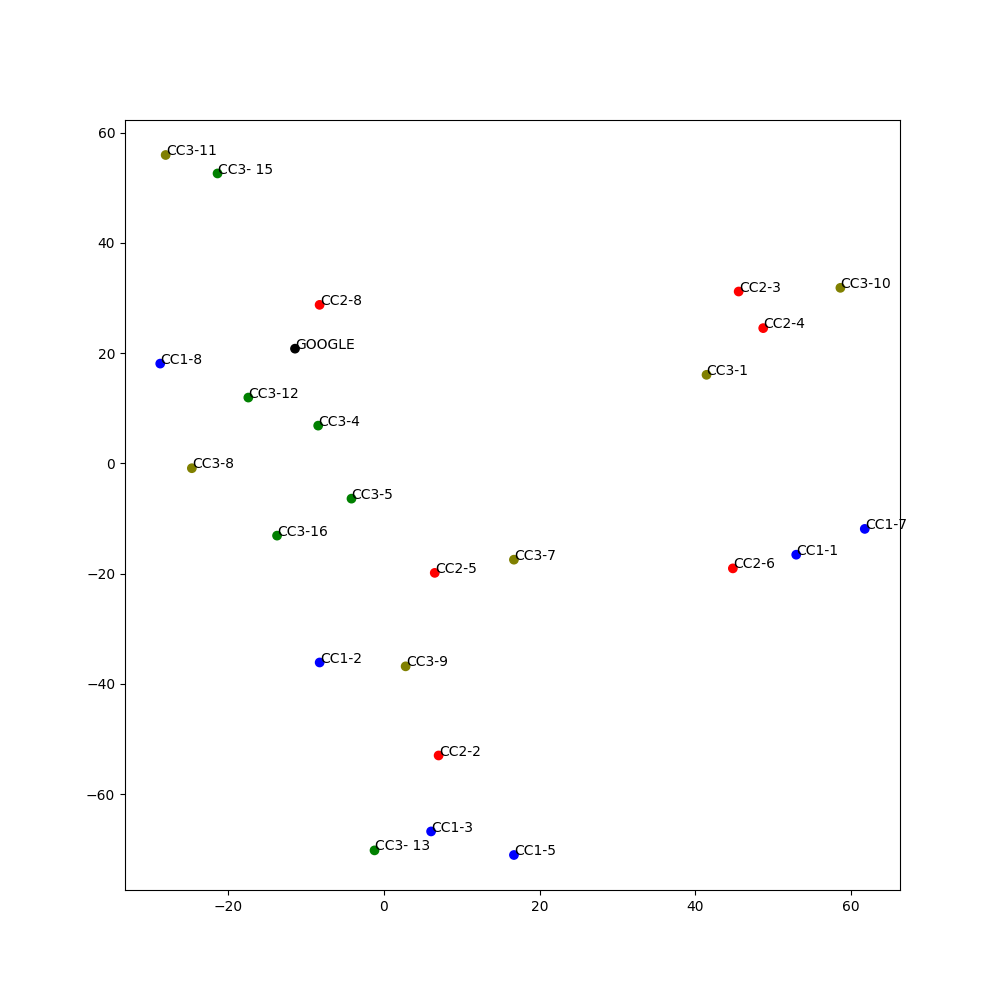
\includegraphics[scale=0.6]{TSNE_normalisé.png}

Dans cette projection les axes ne sont pas interprétables, mais les proximités sont très bien respectées. On peut donc faire les remarques suivantes :
\begin{enumerate}
	\item Il y a un cluster de très bonnes représentations centré autour de la référence, qui contient presque tous les graphes du groupe 3bis (à l'exception à nouveau de 3-13).
	\item On notera que dans chaque groupe il y a quand même une très bonne représentation à chaque fois (respectivement 1-8, 2-8 et 3-8)
	\item Alors que le groupe 3bis est très nettement au-dessus, il n'est pas réellement possible de hiérarchiser les groupes 1, 2 et 3 entre eux à partir de cette méthode. (Nous verrons plus loin une autre méthode qui le permet)
	\item Cependant on constate qu'il y a une forme de cohérence entre les graphes d'un même groupe, c'est-à-dire que même ceux qui sont fortement déformés le sont plus souvent de façon similaire. Ainsi, les graphes du groupe 1 ont tendance à se rapprocher les un des autres (1-3 avec 1-5, 1-1 avec 1-7), de même pour le groupe 2 (2-4 avec 2-3).
\end{enumerate}

Ceci étant, toutes ces conclusions sont à relativiser : compte tenu de la taille faible des groupes, on a quand même une variabilité intra-groupe assez élevée.

\section{Centralité}

Pour procéder à un calcul de centralité sur un graphe complet, il convient d'abord de choisir arbitrairement une mesure de similarité pour les poids des arêtes ; ici nous avons tout simplement pris l'inverse de la distance.\\

\begin{center}
Centralité des sommets

\begin{tabular}{rllllll}
& Q & E & F & M & S & MSH\\
1-5&0,335 & 0,354 & 0,690 & 0,810 & 0,848 & 0,798\\
1-7&0,372 & 0,417 & 1,104 & 0,621 & 0,927 & 0,967\\
1-1&0,531 & 0,624 & 0,905 & 0,694 & 0,846 & 0,969\\
1-2&0,544 & 0,312 & 1,013 & 0,618 & 0,491 & 0,967\\
1-3&0,312 & 0,278 & 0,878 & 0,846 & 0,584 & 0,646\\
1-8&0,379 & 0,355 & 1,322 & 1,251 & 0,853 & 0,943\\
2-2&0,328 & 0,301 & 0,719 & 0,561 & 0,555 & 0,606\\
2-3&0,306 & 0,385 & 1,396 & 1,079 & 0,972 & 1,288\\
2-4&0,306 & 0,373 & 1,090 & 1,022 & 0,891 & 0,986\\
2-5&0,383 & 0,347 & 1,413 & 1,324 & 0,559 & 0,821\\
2-6&0,416 & 0,627 & 0,982 & 0,810 & 0,621 & 0,833\\
2-8&0,378 & 0,344 & 2,448 & 2,137 & 1,072 & 1,758\\
3-1&0,335 & 0,380 & 1,089 & 0,861 & 0,686 & 1,034\\
3-7&0,351 & 0,403 & 1,310 & 1,114 & 0,514 & 1,000\\
3-8&0,393 & 0,288 & 1,242 & 0,968 & 0,705 & 1,063\\
3-9&0,363 & 0,297 & 0,970 & 0,879 & 0,570 & 0,686\\
3-10&0,267 & 0,446 & 1,401 & 1,397 & 0,855 & 0,866\\
3-11&0,320 & 0,260 & 1,426 & 1,027 & 1,349 & 1,476\\
3-4&0,384 & 0,329 & 1,555 & 1,398 & 0,812 & 1,274\\
3-5&0,377 & 0,335 & 1,377 & 1,269 & 0,677 & 0,940\\
3-12&0,360 & 0,306 & 1,923 & 1,704 & 0,779 & 1,280\\
3-13&0,314 & 0,242 & 1,126 & 0,934 & 0,529 & 0,891\\
3-15&0,304 & 0,274 & 1,912 & 1,909 & 1,291 & 1,532\\
3-16&0,362 & 0,301 & 1,205 & 1,072 & 0,595 & 0,855\\
GOOGLE&0,351 & 0,335 & 1,703 & 1,299 & 0,921 & 1,511\\
\end{tabular}
\end{center}

Sans surprise, dans tous les graphes, les noeuds Q et E (Eglise et Quai) ont une faible centralité tandis que les noeuds F et M (Franprix et Métro) en ont une élevée - avec une variance plus importante pour ce dernier.

La centralité des noeuds constitue un espace réduit sur lequel il est possible de construire une nouvelle représentation, par exemple une ACP. Dans celle-ci nous capturons 75\% de la variance sur les deux premiers axes, ce qui en fait une représentation raisonnablement fidèle.

\includegraphics[scale=0.6]{centr_PCA_normalisée_axes0-1.png}

On distingue un axe horizontal (55\% de la variance) qui représente la capacité à bien positionner les noeuds centraux (MSH, métro, Franprix et square), et un axe vertical (20\%) qui représente la capacité à positionner les noeuds excentrés.

Dans cette configuration, on voit que tous les graphes du groupe 1 sous-estiment fortement la centralité des noeuds centraux, y compris le meilleur, 1-8. De surcroît la moitié d'entre eux surestiment celle des noeuds extérieurs, résultant en des graphes beaucoup trop symétriques.

Les graphes du groupe 2 présentent des profils variés, avec tous les types d'erreur représentés.

Les graphes des groupes 3 et 3bis estiment tous à peu près correctement les centralités des noeuds Q et E. En revanche, leurs estimations pour les noeuds centraux présentent une forte variabilité.

D'une façon générale, la grande majorité des modèles sous-estime la centralité des noeuds centraux, en exagérant les distances courtes.


\begin{center}
Centralité moyenne par groupe\\
\begin{tabular}{rllllll}
& Q & E & F & M & S & MSH\\
groupe 1 & \textcolor{red}{\textbf{0.412}} & 0.390 & \textcolor{red}{\textbf{0.985}} & \textcolor{red}{\textbf{0.807}} & 0.758 & \textcolor{red}{\textbf{0.882}}\\
groupe 2 & \textcolor{teal}{\textbf{0.353}} & 0.396 & \textcolor{red}{\textbf{1.342}} & 1.156 & 0.778 & \textcolor{red}{\textbf{1.049}}\\
groupe 3 & 0.338 & \textcolor{teal}{\textbf{0.346}} & \textcolor{red}{\textbf{1.239}} & \textcolor{red}{\textbf{1.041}} & 0.780 & \textcolor{red}{\textbf{1.021}}\\
groupe 3bis & \textcolor{teal}{\textbf{0.350}} & 0.298 & 1.516 & \textcolor{teal}{\textbf{1.381}} & 0.781 & 1.129\\
\textit{GOOGLE} & \textit{0.351} & \textit{0.335} & \textit{1.703} & \textit{1.299} & \textit{0.921} & \textit{1.511}\\
\end{tabular}
\end{center}

\section{Calculs d'aires}

Les représentations de type ACP appliquées aux distances sont par définition des transformations linéaires, utiles pour comprendre la stricte perception des distances. Mais on peut également s'intéresser aux perceptions spatiales, en prenant cette fois comme variables élémentaires les aires des triangles. 

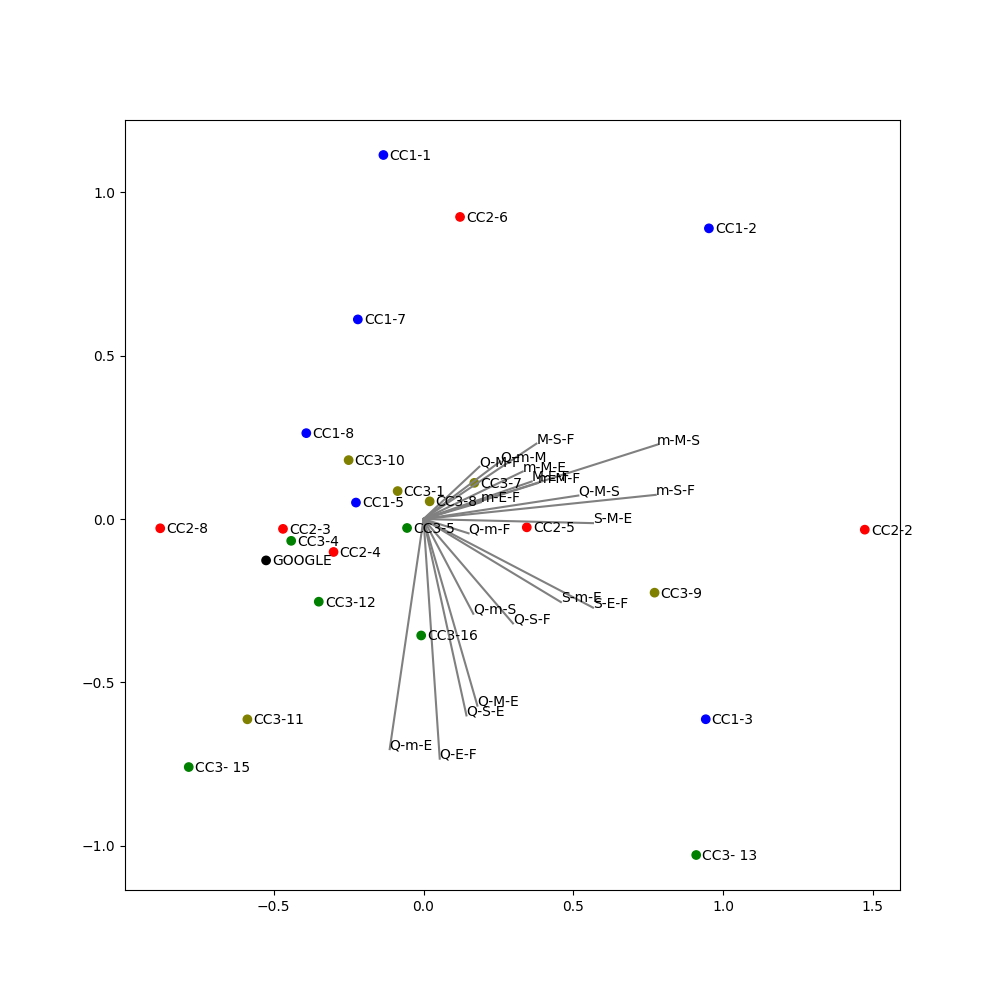
\includegraphics[scale=0.6]{PCA_aires_axes0-1.png}

Ici les deux premiers axes ne capturent respectivement que 29\% et 20\% de la variance (essentiellement parce qu'il y a désormais 20 variables), donc nous figurons également les deux axes suivants (17\% et 8\%) pour ne pas risquer de surinterprétation:

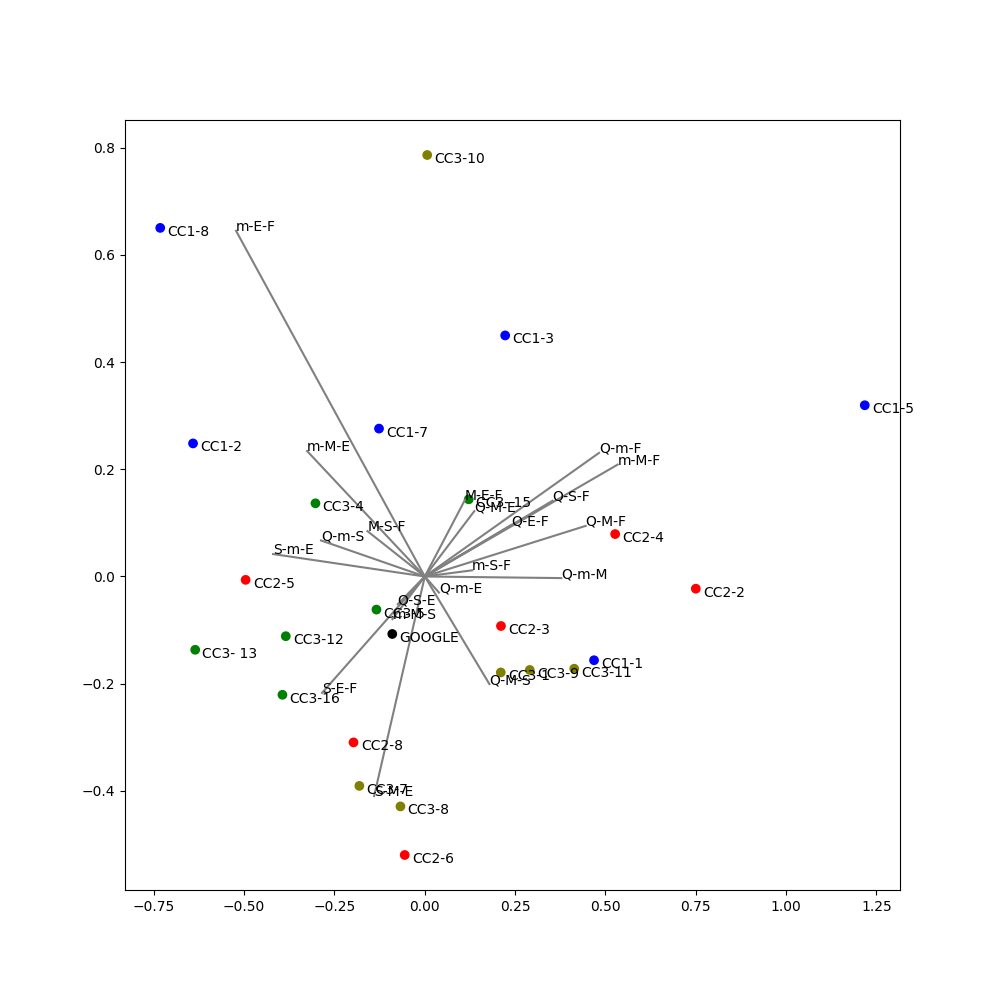
\includegraphics[scale=0.6]{PCA_aires_axes2-3.png}

En regardant simultanément les deux représentations on constate que :
\begin{itemize}
	\item le premier axe (horizontalement dans le premier graphe) élimine surtout quelques graphes très déformés comme 2-2 et 1-2, mais illustre aussi que dans l'ensemble la plupart des graphes surestiment les petites aires.
	\item le second axe (verticalement dans le premier graphe) témoigne du fait que la majorité des plans du groupe 1 (sauf 1-3) sous-estiment les aires des triangles incluant le quai tandis que ceux des groupes 3 et 3bis ont plutôt tendance à les surestimer.
	\item le troisième axe (horizontalement dans le second graphe) caractérise la propension de certains sommets des groupes 1 et 2 à exagérer les aires incluant le Franprix.
	\item enfin le quatrième axe (verticalement dans le second graphe), à ne pas surinterpréter du fait de sa faible contribution, témoigne que le groupe 1 exagère significativement la taille du triangle MSH-Eglise-Fraprix, alors que les groupe 2 et 3bis exagère les aires des triangles incluant le parc.
\end{itemize}



\end{document}
